
Here is what we have learned so far: to use the processor efficiently, we must give it enough code to execute many instructions in parallel. The main reason we may not have enough instructions to keep the CPU busy is the data dependencies: we have the code, but we cannot run it because the inputs aren't ready. We solve this problem by pipelining the code, but in order to do so, we must know in advance which instructions are going to be executed. We cannot do this if we do not know in advance which path the execution will take. The way we deal with that is by making an educated guess about whether a conditional branch will be taken or not, based on the history of evaluating this condition. The more reliable the guess, the better the performance. Sometimes, there is no way to guess reliably, and performance suffers.

The root of all of these performance problems is the conditional branches, where the next instruction to be executed is not known until runtime. A radical solution to the problem would be to rewrite our code to use no branches or at least much fewer of them. This is known as branchless computing.

\subsubsubsection{3.8.1\hspace{0.2cm}Loop unrolling}

In truth, the idea is not particularly novel. Now that you understand the mechanism by which the branches affect performance, you can recognize the well-known technique of loop unrolling as an early example of code transformation for the purpose of reducing the number of branches. Let us go all the way back to our original code example:

\begin{lstlisting}[style=styleCXX]
for (size_t i = 0; i < N; ++i) {
	a1 += p1[i] + p2[i];
}
\end{lstlisting}

We understand now that, while the body of the loop is perfectly pipelined, there is a hidden branch in this code: the end of the loop check. This check is performed once per loop iteration. If we had prior knowledge that, say, the number of iterations N is always even, then we don't need to perform the check after odd iterations. We can explicitly omit this check as follows:

\begin{lstlisting}[style=styleCXX]
for (size_t i = 0; i < N; i += 2) {
	a1 += p1[i] + p2[i]
		+ p1[i+1] + p2[i+1];
}
\end{lstlisting}

We have unrolled this loop, converted two iterations into one larger one. In this and other similar examples, the manual unrolling is not likely to improve performance for several reasons: first of all, the end of the loop branch is predicted almost perfectly if N is large. Second, the compiler may do the unrolling anyway as an optimization; more likely, a vectorizing compiler will use SSE or AVX instructions to implement this loop, which, in effect, unrolls its body since the vector instructions process several array elements at once. All of these conclusions need to be confirmed by benchmarking or profiling; just don't be surprised if you find out that manual loop unrolling had no effect on performance: this does not mean that what we learned about branches is not true; it means that our original code already had the benefit of loop unrolling, thanks to the compiler optimizations most likely.

\subsubsubsection{3.8.2\hspace{0.2cm}Branchless selection}

Loop unrolling is a very specific optimization that the compilers were taught to do. Generalizing this idea into branchless computing is a recent advance that can yield spectacular performance gains. We will start with a very simple example:

\begin{lstlisting}[style=styleCXX]
unsigned long* p1 = ...; // Data
bool* b1 = ...; // Unpredictable condition
unsigned long a1 = 0, a2 = 0;
for (size_t i = 0; i < N; ++i) {
	if (b1[i]) {
		a1 += p1[i];
	} else {
		a2 += p1[i];
	}
}
\end{lstlisting}

Let us assume that the conditional variable b1[i] cannot be predicted by the processor. As we have already seen, this code runs several times slower than a loop with a well-predicted branch. However, we can do even better; we can eliminate the branch entirely and replace it by indexing into an array of pointers to the two destination variables:

\begin{lstlisting}[style=styleCXX]
unsigned long* p1 = ...; // Data
bool* b1 = ...; // Unpredictable condition
unsigned long a1 = 0, a2 = 0;
unsigned long* a[2] = { &a2, &a1 };
for (size_t i = 0; i < N; ++i) {
	a[b1[i]] += p1[i];
}
\end{lstlisting}

In this transformation, we take advantage of the fact that a boolean variable can have only two values, 0 (false) or 1 (true), and is implicitly convertible to an integer (if we used some other type instead of bool, we would have to make sure that all true values are indeed represented by 1 since any non-zero value is considered true but only the value of 1 works in our branchless code).

This transformation replaces a conditional jump to one of two possible instructions by conditional access of one of two possible memory locations. Because such conditional memory accesses can be pipelined, the branchless version delivers significant performance improvement:

\hspace*{\fill} \\ %插入空行
\begin{center}
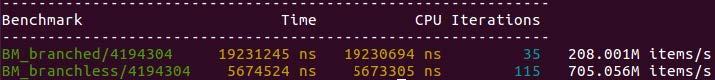
\includegraphics[width=0.9\textwidth]{content/1/chapter3/images/30.jpg}\\
Figure 3.30
\end{center}

In this example, the branchless version of the code is 3.5 times faster. It is worth noting that some compilers implement the ?: operator using a lookup array instead of a conditional branch whenever possible. With such a compiler, we can gain the same performance benefit by rewriting our loop body as follows:

\begin{lstlisting}[style=styleCXX]
for (size_t i = 0; i < N; ++i) {
	(b1[i] ? a1 : a2) += p1[i];
}
\end{lstlisting}

As usual, the only way to be certain whether this optimization works or how effective it is, is to measure.

The preceding example covers all essential elements of branchless computing: instead of conditionally executing this code or that code, we transform the program so that the code is the same in all cases, and the conditional logic is implemented by an indexing operation. We will go through several more examples to highlight some noteworthy considerations and limitations.

\subsubsubsection{3.8.3\hspace{0.2cm}Branchless computing examples}

Most of the time, the code that depends on the condition is not as simple as where to write the result. Usually, we have to do the computations differently depending on some intermediate values:

\begin{lstlisting}[style=styleCXX]
unsigned long *p1 = ..., *p2 = ...; // Data
bool* b1 = ...; // Unpredictable condition
unsigned long a1 = 0, a2 = 0;
for (size_t i = 0; i < N; ++i) {
	if (b1[i]) {
		a1 += p1[i] - p2[i];
	} else {
		a2 += p1[i] * p2[i];
	}
}
\end{lstlisting}

Here the condition affects what expression we compute and where the result is stored. The only thing common to both branches is the input, and even that doesn't have to be the case, in general.

To compute the same results without branches, we have to fetch the result of the correct expression from a memory location indexed by the condition variable. This implies that both expressions will be evaluated since we decided not to change which code we execute based on the condition. With this understanding, the transformation to the branchless form is straightforward:

\begin{lstlisting}[style=styleCXX]
unsigned long a1 = 0, a2 = 0;
unsigned long* a[2] = { &a2, &a1 };
for (size_t i = 0; i < N; ++i) {
	unsigned long s[2] = { p1[i] * p2[i], p1[i] - p2[i] };
	a[b1[i]] += s[b1[i]];
}
\end{lstlisting}

Both expressions are evaluated, and their results are stored in an array. Another array is used to index the destination of the computation, that is, which variable is incremented. Overall, we have significantly increased the amount of computing the loop body must do; on the other hand, it's all sequential code with no jumps, so, as long as the CPU has the resources to do few more operations without spending any extra cycles, we should come out ahead. The benchmark confirms that indeed this branchless transformation is effective:

\hspace*{\fill} \\ %插入空行
\begin{center}
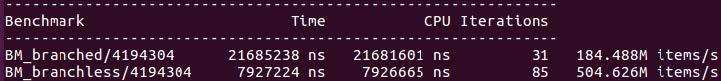
\includegraphics[width=0.9\textwidth]{content/1/chapter3/images/31.jpg}\\
Figure 3.31
\end{center}

It must be stressed that there is a limit to how many extra computations you can do and still outperform the conditional code. There isn't even a good general rule of thumb you could use to make an educated guess here (and you should never guess about performance anyway). The effectiveness of such optimizations must be measured: it is highly dependent on both the code and the data. For example, if the branch predictor were highly effective (predictable condition instead of a random one), the conditional code would outperform the branchless version:

\hspace*{\fill} \\ %插入空行
\begin{center}
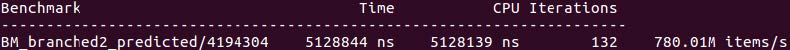
\includegraphics[width=0.9\textwidth]{content/1/chapter3/images/32.jpg}\\
Figure 3.32
\end{center}

Perhaps the most remarkable conclusion we can learn from Figure 3.31 and Figure 3.32 is just how expensive a pipeline flush (a mispredicted branch) is and how much computing the CPU can do at once with instruction-level parallelism. The latter can be deduced from the relatively small difference in performance between the perfectly predicted branch (Figure 3.32) and the branchless implementation (Figure 3.31). This hidden and largely unused reserve of computing power is what branchless computing relies on, and we probably have not exhausted this reserve in our example. It is instructive to show another variant of the branchless transformation of the same code where, instead of using an array to select the right result variable, we always increment both by zero if we don't want to actually change the result:

\begin{lstlisting}[style=styleCXX]
unsigned long a1 = 0, a2 = 0;
for (size_t i = 0; i < N; ++i) {
	unsigned long s1[2] = { 0, p1[i] - p2[i] };
	unsigned long s2[2] = { p1[i] * p2[i], 0 };
	a1 += s1[b1[i]];
	a2 += s2[b1[i]];
}
\end{lstlisting}

Instead of an array of destinations, we now have two arrays of intermediate values. This version does even more computations unconditionally and yet, provides the same performance as the previous branchless code:

\hspace*{\fill} \\ %插入空行
\begin{center}
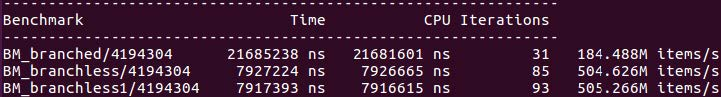
\includegraphics[width=0.9\textwidth]{content/1/chapter3/images/33.jpg}\\
Figure 3.33 – The results of Figure 3.31, with the alternative branchless implementation added as "BM\_branchless1"
\end{center}

It is important to understand the limitations of the branchless transformations and not get carried away. We have already seen the first limitation: branchless code usually executes more instructions; therefore, if the branch predictor ends up working well, the small number of pipeline flushes may not be enough to justify the optimization.

The second reason for the branchless transformation to not perform as expected has to do with the compiler: in some cases, the compiler can do an equivalent or even better optimization. For example, consider what is known as a clamp loop:

\begin{lstlisting}[style=styleCXX]
unsigned char *c = ...; // Random values from 0 to 255
for (size_t i = 0; i < N; ++i) {
	c[i] = (c[i] < 128) ? c[i] : 128;
}
\end{lstlisting}

This loop clamps the values in an array c of unsigned char to the limit of 128. Assuming the initial values were random, the condition in the body of the loop cannot be predicted with any degree of certainty, and we can expect a very high branch misprediction rate. The alternative, branchless, implementation uses a lookup table (LUT) that has 256 elements, one for each possible value of unsigned char. The table entries LUT[i] for indices i from 0 to 127 contain the index value itself, and the entries LUT[i] for the higher indices all contain 128:

\begin{lstlisting}[style=styleCXX]
unsigned char *c = ...; // Random values from 0 to 255
unsigned char LUT[256] = { 0, 1, …, 127, 128, 128, … 128 };
for (size_t i = 0; i < N; ++i) {
	c[i] = LUT[c[i]];
}
\end{lstlisting}

With most modern compilers, this is not optimization at all: the compiler will do better with the original code, most likely using SSE or AVX vector instructions to copy and clamp multiple characters at once and without any branches at all. If we profiled the original code instead of assuming that the branch must be mispredicted, we would have discovered that the program does not suffer from a poor branch prediction.

There is one more scenario where a branchless transformation may not pay off, and that is the case when the body of the loop is significantly more expensive than the branch, even a mispredicted one. This case is notable because it often describes loops that make function calls:

\begin{lstlisting}[style=styleCXX]
unsigned long f1(unsigned long x, unsigned long y);
unsigned long f2(unsigned long x, unsigned long y);
unsigned long *p1 = ..., *p2 = ...; // Data
bool* b1 = ...; // Unpredictable condition
unsigned long a = 0;
for (size_t i = 0; i < N; ++i) {
	if (b1[i]) {
		a += f1(p1[i], p2[i]);
	} else {
		a += f2(p1[i], p2[i]);
	}
}
\end{lstlisting}

Here we call one of the two functions, f1() or f2(), depending on the condition b1. The if-else statement can be eliminated, and the code can be made branchless if we use an array of function pointers:

\begin{lstlisting}[style=styleCXX]
decltype(f1)* f[] = { f1, f2 };
for (size_t i = 0; i < N; ++i) {
	a += f[b1[i]](p1[i], p2[i]);
}
\end{lstlisting}

Is this an optimization worth doing? Often, it isn't. First of all, if the functions f1() or f2() can be inlined, the function pointer call will prevent that. Inlining is usually a major optimization; giving up inlining to get rid of a branch is almost never justified. When the functions are not inlined, the function call by itself disrupts the pipeline (this is one reason inlining is such an effective optimization). Compared to the cost of the function call, even a mispredicted branch is usually not that much.

Nonetheless, sometimes this function lookup table is a worthwhile optimization: it almost never pays off for just two alternatives, but if we had to choose from many functions based on a single condition, the function pointer table is more efficient than a chained if-else statement. It is worth noting that this example is very similar to the implementation used by all modern compilers to implement virtual function calls; such calls are also dispatched using an array of function pointers instead of a chain of comparisons. When faced with a need to optimize code that calls one of several functions based on a runtime condition, you should consider whether a redesign using polymorphic objects is worthwhile.

You should also keep in mind the effect of the branchless transformations on the readability of your code: a lookup table of function pointers is not as easy to read and can be much harder to debug than a switch or if-else statement. Given the many factors contributing to the final outcome (compiler optimizations, hardware resource availability, the nature of the data the program operates on), any optimizations must be verified by measurements such as benchmarks and profiles and weighed against the additional cost imposed on the programmer in terms of time, readability, and complexity.








